% This LaTeX was auto-generated from MATLAB code.
% To make changes, update the MATLAB code and export to LaTeX again.

\documentclass{article}

\usepackage[utf8]{inputenc}
\usepackage[T1]{fontenc}
\usepackage{lmodern}
\usepackage{graphicx}
\usepackage{color}
\usepackage{hyperref}
\usepackage{amsmath}
\usepackage{amsfonts}
\usepackage{epstopdf}
\usepackage[table]{xcolor}
\usepackage{matlab}

\sloppy
\epstopdfsetup{outdir=./}
\graphicspath{ {./lab2_images/} }

\begin{document}

\begin{matlabcode}
% Import the voltage measurements from the OScope
voltage_readings = readtable("thermistor.csv");

% Symbolically solve for the resistance of the thermistor
% V_out = V_in * (R_2 / R_2 + R_thermistor)
syms V_out V_in R_2 R_thermistor;
eqn_R = V_out == V_in * (R_2 / (R_2 + R_thermistor))
\end{matlabcode}
\begin{matlabsymbolicoutput}
eqn\_R = 

\hskip1em $\displaystyle V_{\textrm{out}} =\frac{R_2 \,V_{\textrm{in}} }{R_2 +R_{\textrm{thermistor}} }$
\end{matlabsymbolicoutput}
\begin{matlabcode}
S_R = solve(eqn_R, R_thermistor)
\end{matlabcode}
\begin{matlabsymbolicoutput}
S\_R = 

\hskip1em $\displaystyle \frac{R_2 \,V_{\textrm{in}} }{V_{\textrm{out}} }-R_2 $
\end{matlabsymbolicoutput}
\begin{matlabcode}

% Experiment set up input
V_in = 5;
R_2 = 301;

% Using Ohm's Law
func_R = @(V_out) ((R_2*V_in) / V_out) - R_2;

% Calculate the resistance according to the changes in the voltage
% measurements
voltage_readings.R_thermistor = rowfun( ...
    func_R, voltage_readings(:, 2), 'OutputFormat', 'uniform' ...
    );

% Symbolically solve for the temperature with the given calibration 
% eqn for the thermistor:
% Resitstance = 1000 Ohm * e^(-3528 * ((1/298)-(1/Temperature)))
syms T
eqn_temp = R_thermistor == 1000 * exp(-3528 * ((1/298) - (1/T)))
\end{matlabcode}
\begin{matlabsymbolicoutput}
eqn\_temp = 

\hskip1em $\displaystyle R_{\textrm{thermistor}} =1000\,{\mathrm{e}}^{\frac{3528}{T}-\frac{1764}{149}} $
\end{matlabsymbolicoutput}
\begin{matlabcode}
S_temp = solve(eqn_temp, T)
\end{matlabcode}
\begin{matlaboutput}
Warning: Solutions are only valid under certain conditions. To include parameters and conditions in the solution, specify the 'ReturnConditions' value as 'true'.
\end{matlaboutput}
\begin{matlabsymbolicoutput}
S\_temp = 

\hskip1em $\displaystyle \frac{1}{\frac{\log \left(\frac{R_{\textrm{thermistor}} }{1000}\right)}{3528}+\frac{1}{298}}$
\end{matlabsymbolicoutput}
\begin{matlabcode}

% Calculating the temperature numerically using the calculated resistance
% of the thermistor
func_temp = @(R_thermistor) 1 / ((log(R_thermistor/1000)/3528) + 1/298);
voltage_readings.Temperature = rowfun( ...
    func_temp, ...
    voltage_readings(:,5), ...
    'ExtractCellContents', 1, ...
    'OutputFormat', 'uniform' ...
    );

% Plotting Temperature vs Time
clf
plot(voltage_readings{:, 1} + 375, voltage_readings{:, 6}); hold on
axis([0 380 320 360])
title("Temperature vs Time")
xlabel("Time (sec)")
ylabel("Temperature (K)")
yline(340.6, '-.r')
yline(356.5, '-.r')
yline(324.5, '-.r')
yyaxis right
yticks([0.05 0.7])
yticklabels ({'\DeltaT_2=-4.4K', '\DeltaT_1=-15.9K'})
hold off
\end{matlabcode}
\begin{center}
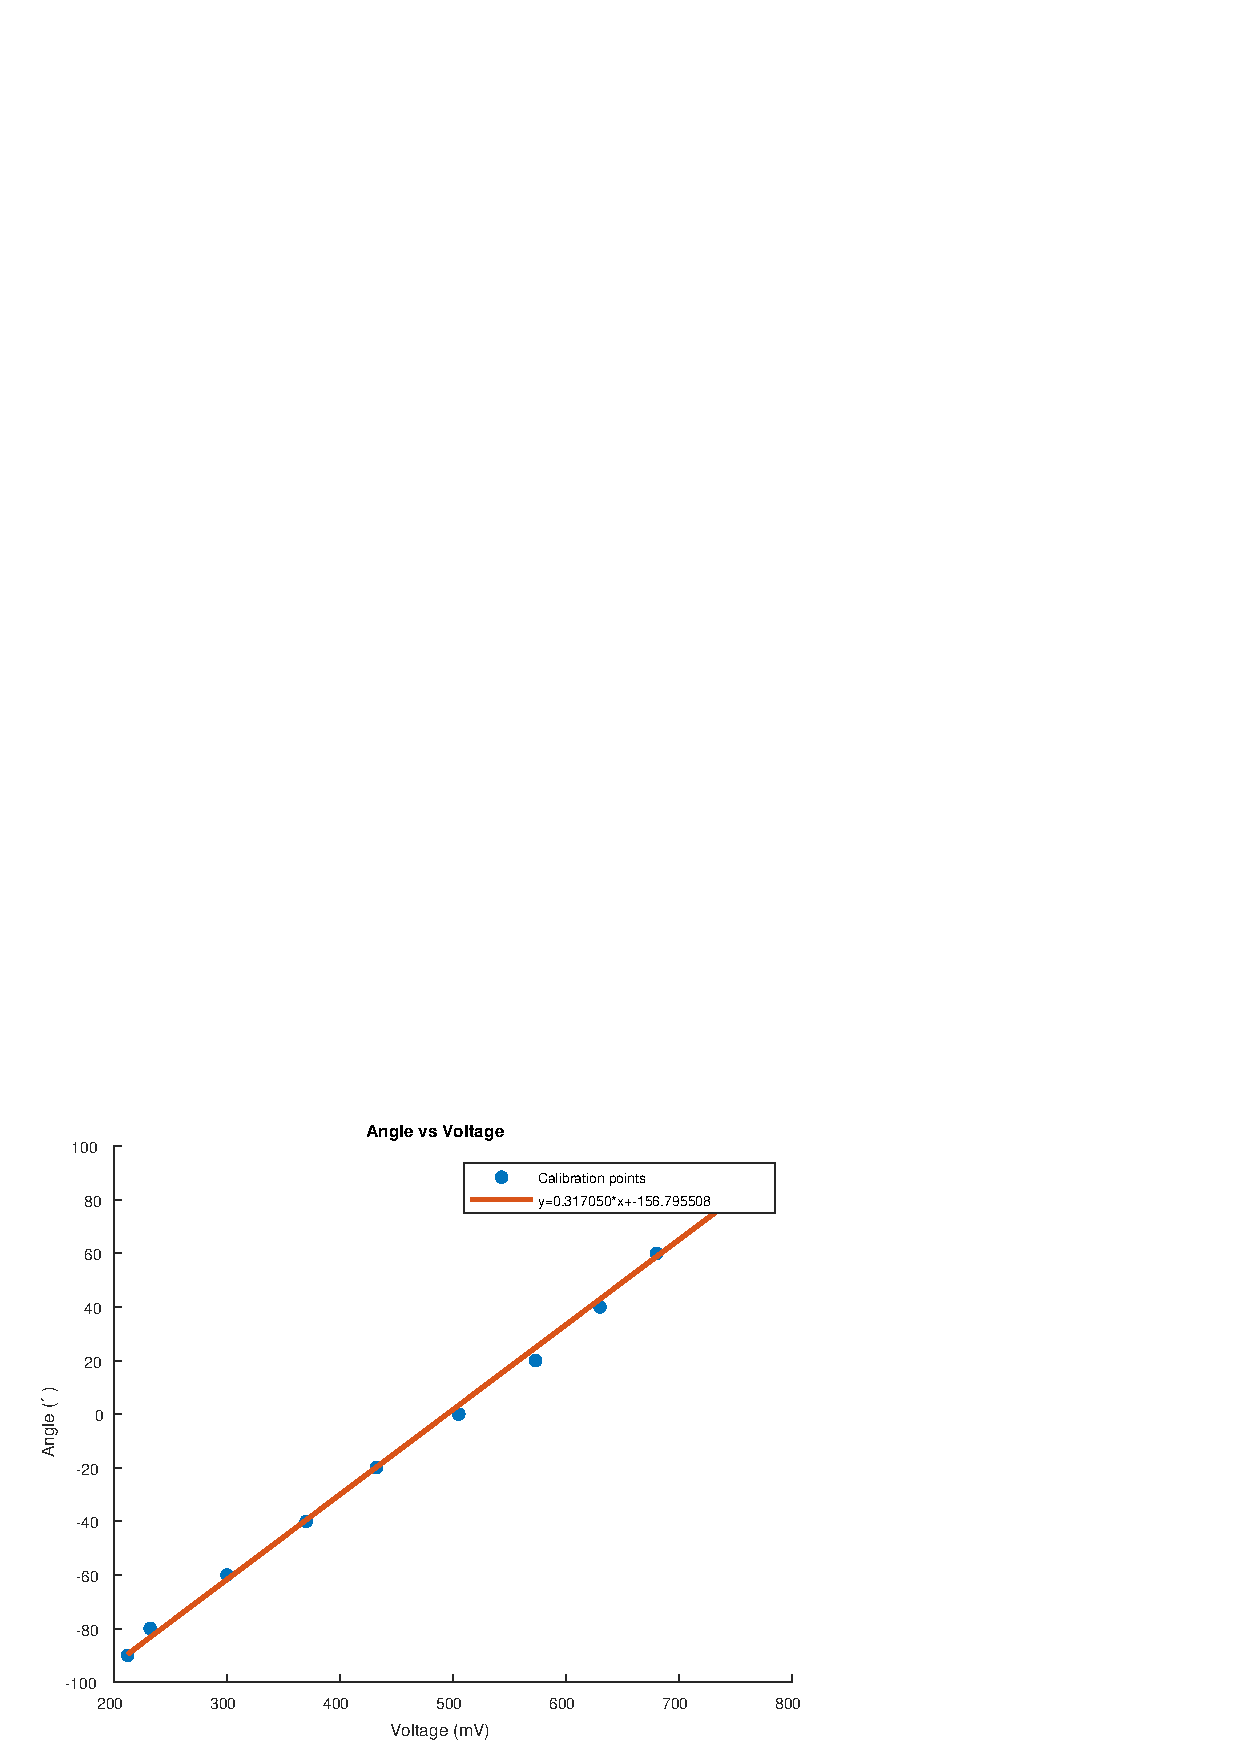
\includegraphics[width=\maxwidth{56.196688409433015em}]{figure_0.png}
\end{center}
\begin{matlabcode}




\end{matlabcode}

\end{document}
